\section{Beat the Machine}
\label{sec:btm}

% \josh{ensure that the language matches the earlier motivation in secs 2 and 3}

Assessing the in-the-wild performance of any automated classification system can be a challenge. Situations with class imbalance and rare disjunctive sub-concepts such as the hate speech classifier presented in Section~\ref{sec:intro} make accurate assessment particularly difficult and lead to the existence of unknown unknowns. Traditionally, we would sample from the output decisions and employ humans to verify the correctness of the classifications.  Using these judgments we can estimate the error rate in different parts of the classification space. Unfortunately, given our problem characteristics, the process can be woefully inefficient. First, if the classification decisions are relatively accurate, then most of the results will be accurate, and without intelligent sampling, humans will encounter errors very infrequently. Second, if there is substantial class imbalance, most of the encountered errors would be misclassifications of majority-class examples  into the minority; this is problematic, since in significantly imbalanced classification problems, the minority class generally incurs a far greater mistake cost---as in the case of hate speech, this is what is being predicted. Third, if the problem space has rare disjunctive sub-concepts, identification may be particularly tricky---chances of occurrence may be $1:1,000,000$ or less. In these situations, it can become quite difficult to identify misclassifications of examples whose true class is the minority class. 

\begin{xmpl} Consider the case of identifying pages with hate speech content. If we have a relatively accurate classifier, with 95\% accuracy on each class, it becomes very difficult to identify misclassified pages that contain hate speech. In a random sample, most of the pages are correctly classified as benign. Even in the unrealistically generous case that 
0.1\% of the pages on the Internet contain such objectionable content, to find one ``false negative'' (the severe error: hate speech passing as benign) we will have to inspect approximately $20,000$ pages (and in the process would find around $1,000$ false positives). \smartqed

%This is echoed in the   performance of the ``random labeling'' used to generate the $k$-NN model presented in Figure~\ref{fig:uuvsku}. 
\end{xmpl} 

 %In reality, far less than 0.1\% of the pages on the Internet contain such content.

It is tempting to consider such problems inconsequential. However, when such a system is used to filter billions of pages, such ``relatively infrequent'' errors become frequent in absolute numbers. Furthermore, even one-off cases can cause significant damage, for example, to the public image of a company that accidentally supports a site containing such content through advertising. Unknown unknowns may be particularly damaging; client's expectations haven't been properly managed, and detailed contingencies are unlikely to exist. 

Instead of passively waiting for such unknown errors to ``emerge'' we can instead actively seek to find them. We describe a system that engages human intelligence, accessed through crowdsourcing, to identify these unknown unknown cases. In a sense, this is similar to ``white hat'' hackers who are hired by companies to find vulnerabilities and break into their own security systems. In our case, human workers are asked to submit pages that will ``beat'' our classifier.

\subsection{Beat the Machine Task Design}

The BTM system has evolved over time. We will walk through several design iterations, showing the challenged that emerged with each new design, and how these challenges were addressed. 

\textbf{Design 1, Initial version}: Let's start with a straightforward idea: Ask humans to find the unknown unknowns, i.e., the cases that ``beat the machine''---the users  submit URLs that they believe will be incorrectly classified by the current classification model.  To spur engagement, a user receives a nominal payment for just submitting the URLs, and then she receives a significant bonus payment for every URL that was misclassified. (In the implementation, the nominal payment was 1 cent per 5 URLs, and the payment per misclassified URL is 20 cents.)  

Of course there is an obvious problem: how could such a system tell that the URL indeed beats the machine.  The whole point is to find cases that the system does not know that it gets wrong!   To judge misclassification, we task another set of (trusted) humans to classify these URLs.  Then, to determine whether the URL beats the machine, we compare the classification of the trusted set of humans with the outcome of the machine model. To avoid certain issues of gaming, the BTM workers are recruited through Amazon Mechanical Turk, and the trusted human judges are recruited and trained through oDesk for the fully automated system. For the experimental evaluation, we used student interns using a separate system.  Unfortunately, this simple design is not as effective as we would have liked, for a variety of reasons.

The first, and most obvious, problem is the lack of interactivity.  The workers can easily submit URLs that would break the model, but then they have to wait for other humans to inspect the results, in order to assess whether they had succeeded. This process can take from a few minutes to a few hours. The delay made the task opaque to the players of the BTM game,
as they do not know if they are good in ``playing the game'' or not. This leads to a short user engagement, and high rates of abandonment.

\textbf{Design 2, Adding immediate classification feedback}: To resolve (partially) the lack of interactivity, we augmented the system to classify URLs on the fly, and give immediate feedback to the humans about the classifier outcome. For example ``The machine believes that this URL contains hate speech.  Do you believe that this is correct?'' The BTM player can then decide whether the URL is indeed a misclassification case and submit it for further consideration. Upon submission, the user receives provisional bonus points that correspond to a cash reward. The bonus points become permanent, and the worker is paid, immediately after the inspection and verification of the submitted content by the human judges.
  

Unfortunately, this design still does not provide the proper incentives. Players typically find it much easier to locate pages from the majority class misclassified into the minority (e.g., pages without any hate speech content that are misclassified as containing hate speech). So, instead of locating the desired, high-cost errors, we receive the type of errors that we can find more easily by observing the positive classifications.  Recall that due to the class imbalance, most of the observed errors are good pages being classified as containing hate speech. As described above, we are particularly interested in finding pages that contain hate speech but are incorrectly classified as benign.  And especially, among these, the unknown unknowns. Furthermore, we experience a significant number of cheating attempts where users are submitting random URLs and always insisting that the content is different than the classification decisions, even though the classifier is correct.

\begin{figure}[t]
\center{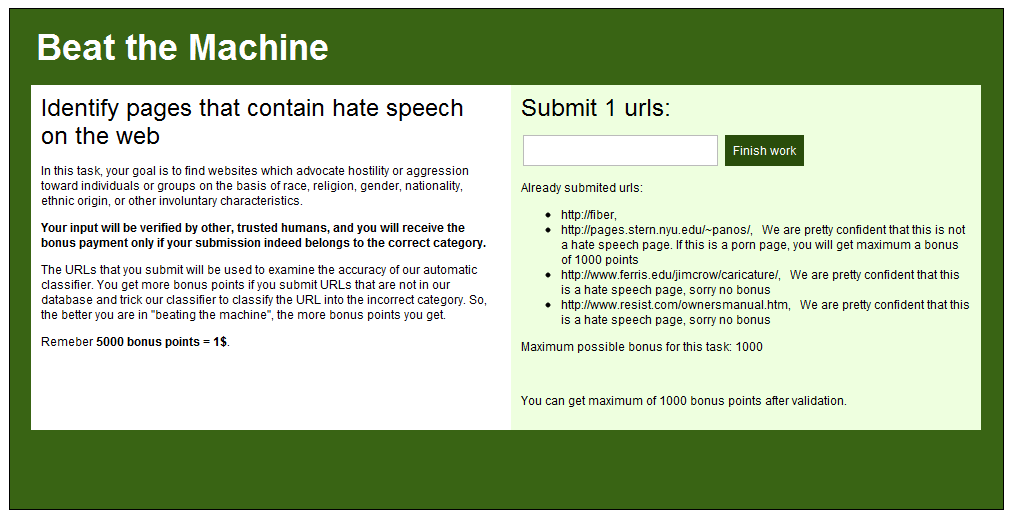
\includegraphics[width=\columnwidth]{plots/btm-HIT.png}}
\caption{A screen-shot of the BTM interface on Mechanical Turk.}
\label{fig:btm}
\end{figure}

\textbf{Design 3, Segmenting the task by class}: To deal with these problems, we split the task into two subtasks: (a)~Seek pages in the minority class that are misclassified in the majority class,\footnote{For example, pages that contain offensive content but are classified as benign.} and (b)~seek pages with benign content that are classified as offensive. This segmentation simplifies the overall design and makes the task easier for participants to understand.  Moreover, it allowed us to quickly reject submissions that are of no interest.  For example, if we are asking for misclassified hate speech pages, we can quickly reject pages that our classifier unambiguously classifies as hate speech. (In the Designs 1 and 2, users had the incentive to mark these as ``non-hate-speech'' hoping that the human judge would accept their judgments.) Figure~\ref{fig:btm} shows the, intentionally simple, task interface. 

\textbf{Design 4, Expanding the incentives}: In this design , we improve the incentive structure by rewarding differently users that discover ``big mistakes'' (the unknown unknowns) and those that discover the ``small mistakes'' (the known unknowns). Instead of giving a constant bonus to the player for a misclassified URL, we reward misclassifications proportionally to the estimated cost, which we infer through the returned probability distribution for the example label.  
For examples that have high estimated cost, the reward is small: this was a known unknown.
On the other hand, if the model is very confident in its decision (i.e., estimated cost close to 0) but the decision is incorrect, then the BTM system gives the highest possible bonus to the worker.\footnote{For the experiments, the highest bonus per URL was worth 1000 points, or 20 cents.} If the the estimated misclassification cost is higher, then the reward is proportionally smaller. We also reward players that provide examples for which the model is correct but uncertain: if the model predicted that the page is 60\% likely to contain hate speech, and the page indeed contained hate speech, the user receives a small bonus.

\textbf{Design 5, Encouraging diversity}:  Design 4 has most of the incentives in place for users to try to discover unknown uknowns. The key problem is what happens after the 
discovery of the first unknown uknowns. Users are typically able to understand what is 
the cause of the failure, and then keep submitting cases that are similar to the previously submitted successes. For example, for the web classification task, users
realized that the classifier was trained with English web sites, and therefore
adult or hate speech sites written in languages other than English (Japanese, German, Arabic, etc.) are effectively unknown unknowns.\footnote{Since most of the terms in non-English websites were not in the training data, the classifier had very few features to work with, and effectively classified these sites into the majority class.} Users realize the vulnerability and then keep submitting similar sites, retrieving high rewards for very little effort. However, once we receive the first few submissions of such unknown unknowns, the similar submissions are only technically unknown unknowns. In reality they become effectively ``known'' unknowns \emph{to the stakeholders}, although for the classification system and BTM they remain unknown uknowns. 

To avoid this issue, we altered the setting to include one additional binary classifier: This extra classifier receives the probe from the user and decides whether the submitted probe is going to be a succesful probe or not. We train this classifier using the previously submitted probes (that were either succesful or not), so this classifier effectively determines whether the current probe is similar to a previously submitted, succesful one. If the classifier determines that the probe is similar to a previously submitted succesful probe, the user receives a smaller reward compared to the case of submitting for the first time an unknown unknown.




